\appendix

\section{Dataset Details}
\label{app:dataset_details}

This appendix documents the schema, selection rules, construction counts, lineage, and descriptive statistics supporting Section~\ref{sec:dataset_patent_reference}--\ref{sec:dataset_synthetic_expansion}. Counts are taken from the finalized patent snapshot, the consolidated synthetic-data processing summary, and the canonical dataset manifests used in the reported experiments.

\subsection{Canonical Schema and CodeV Annotations}
\label{app:dataset_schema}

The canonical table preserves the optical prescription, simulation specification, evaluated descriptors, and provenance in separate column groups. In Table~\ref{tab:canonical_column_groups}, \texttt{XY} denotes a zero-based surface index and \texttt{0X} denotes a field or wavelength index. Empty surface-indexed cells outside the active surface count represent structural absence rather than missing measurements.

\small
\begin{longtable}{@{}p{0.22\textwidth}p{0.25\textwidth}p{0.46\textwidth}@{}}
\caption{Principal column groups in the canonical optical-prescription table.}\label{tab:canonical_column_groups}\\
\toprule
\textbf{Columns or pattern} & \textbf{Quantity} & \textbf{Units and role} \\
\midrule
\endfirsthead
\multicolumn{3}{l}{\textit{Table~\thetable\ continued}}\\
\toprule
\textbf{Columns or pattern} & \textbf{Quantity} & \textbf{Units and role} \\
\midrule
\endhead
\midrule
\multicolumn{3}{r}{\textit{Continued on next page}}\\
\endfoot
\bottomrule
\endlastfoot
\texttt{sXY\_00} & Signed surface radius of curvature & Prescription length unit recorded by \texttt{dim}; primary surface-geometry variable. \\
\texttt{sXY\_01} & Axial distance to the next surface & Prescription length unit recorded by \texttt{dim}; primary surface-geometry variable. \\
\texttt{sXY\_02} & Material following the surface & Catalog label or air; primary surface-material variable. \\
\texttt{sXY\_cir\_00} & Circular aperture semi-diameter & Prescription length unit recorded by \texttt{dim}; evaluated or supplied surface aperture. \\
\texttt{sXY\_k\_00}, \texttt{sXY\_[a--j]\_00} & Conic constant and even-order $A_4$--$A_{20}$ coefficients & Retained for aspheric source designs; absent from the all-spherical canonical subset. \\
\texttt{xan00\_0X}, \texttt{yan00\_0X} & Chief-ray field angle & degrees; one supported field-specification convention. \\
\texttt{xri00\_0X}, \texttt{yri00\_0X}; \texttt{xim00\_0X}, \texttt{yim00\_0X}; \texttt{xob00\_0X}, \texttt{yob00\_0X} & Real-image, paraxial-image, or object-height field specification & mm; alternative source-dependent field conventions. Only the convention used by a design is populated. \\
\texttt{fldx\_0X}, \texttt{fldy\_0X} & Evaluated half field of view & degrees at the reference wavelength. \\
\texttt{wl00\_0X}, \texttt{wtw00\_0X}, \texttt{ref00\_00} & Wavelength, relative weight, and reference-wavelength index & nm, unitless weight, and one-based index, respectively. \\
\texttt{so00\_*}, \texttt{si00\_*} & Object- and image-surface prescription & Radius and axial distance use the prescription length unit recorded by \texttt{dim}; material fields follow the physical-surface convention. \\
\texttt{epd}, \texttt{fno}, \texttt{sto}, \texttt{dim} & Aperture and global setup & Entrance-pupil diameter in the recorded prescription length unit, f-number, stop-surface index, and prescription length unit. \\
\texttt{efl}, \texttt{bfl}, \texttt{oal}, \texttt{lens2img}, \texttt{totlenstrack}, \texttt{objdist}, \texttt{minlenssep}, \texttt{diy} & First-order, packaging, object-distance, separation, and distortion descriptors & Distance-valued fields use the prescription length unit recorded by \texttt{dim}; evaluated by CodeV or derived analytically as appropriate. \\
\texttt{elemcount}, \texttt{cemlenscount}, \texttt{asphcount}, \texttt{surfcount}, \texttt{isintstop} & Structural descriptors & Counts and an internal-stop indicator. \\
\texttt{spo67\_0X}, \texttt{spo100\_0X} & Centroid-referenced polychromatic RMS and full geometric spot diameters & Prescription length unit recorded by \texttt{dim}; diffraction excluded. \\
\texttt{ee50\_0X}, \texttt{ee90\_0X} & Centroid-referenced polychromatic encircled-energy measures & Diffraction-aware CodeV outputs; normalized by Airy diameter for the comparisons in this paper. \\
\texttt{nomperf\_0X} & RMS wavefront aberration & waves at the reference wavelength. \\
\texttt{perfsens\_0X}, \texttt{tolsens\_0X}, \texttt{normalignsens} & Performance, relative tolerance, and alignment sensitivity annotations & CodeV evaluation outputs retained for analysis; they are not generative-model inputs or primary outcome metrics in this study. \\
\texttt{Seq File}, \texttt{dataset\_row\_id}, source-, parent-, perturbation-, and split-related columns & Artifact identity and provenance & Connects each table row to its sequence file, source record, patent family, perturbation record, and benchmark partition. \\
\end{longtable}
\normalsize

In the full patent-derived corpus, the prescription length unit is recorded for each row by \texttt{dim}. The shortlisted patent and synthetic tables are standardized to millimeters. Unless otherwise stated, angles are reported in degrees and wavelengths in nanometers. Optical-performance annotations are excluded from the model-facing feature matrices and used only for filtering, characterization, or post-simulation evaluation.

\subsection{Synthetic Lineage and Traceability}
\label{app:synthetic_lineage_details}

Table~\ref{tab:perturbation_method_counts} reports the final synthetic rows by perturbation family.

\begin{table}[htbp]
\centering
\small
\caption{Perturbation lineage in the final synthetic dataset.}
\label{tab:perturbation_method_counts}
\begin{tabular}{lrr}
\toprule
\textbf{Perturbation method} & \textbf{Rows} & \textbf{Fraction} \\
\midrule
Thickness & 226,846 & 20.2\% \\
Curvature & 185,299 & 16.5\% \\
Thickness + curvature & 179,298 & 15.9\% \\
Material & 140,534 & 12.5\% \\
Thickness + material & 133,733 & 11.9\% \\
Curvature + material & 129,943 & 11.5\% \\
Thickness + curvature + material & 129,427 & 11.5\% \\
\bottomrule
\end{tabular}
\end{table}

The canonical tables retain the lineage groups in Table~\ref{tab:traceability_fields}. These fields remain outside the default model-facing matrices and support source auditing, family-safe splitting, and post-hoc stratification.

\begin{table}[htbp]
\centering
\small
\caption{Traceability fields retained with canonical rows.}
\label{tab:traceability_fields}
\begin{tabular}{@{}p{0.25\linewidth}p{0.67\linewidth}@{}}
\toprule
\textbf{Field group} & \textbf{Representative columns} \\
\midrule
Dataset identity & \texttt{dataset\_row\_id}, \texttt{source\_type}, and \texttt{split}. \\
Source record & \texttt{source\_folder}, \texttt{source\_row\_id}, \texttt{source\_regen\_csv}, and \texttt{source\_submitted\_csv}. \\
Sequence file & \texttt{Seq File}, \texttt{source\_seq\_file\_index}, and \texttt{source\_seq\_file\_basename}. \\
Patent parent & \texttt{parent\_patent\_id}, \texttt{parent\_patent\_row\_id}, and \texttt{parent\_patent\_seq\_file\_basename}. \\
Perturbation & \texttt{perturb\_seed}, \texttt{perturb\_method}, and the curvature-, thickness-, and material-use indicators. \\
Canonical filtering & \texttt{passes\_common\_filters}, \texttt{rejection\_reasons}, and \texttt{filter\_drop\_*}. \\
\bottomrule
\end{tabular}
\end{table}

\subsection{Dataset Characteristics}
\label{app:dataset_characteristics}

Table~\ref{tab:appendix_dataset_characteristics} summarizes the principal ranges. Figures~\ref{fig:appendix_surface_count_distribution} and~\ref{fig:appendix_condition_distributions} compare topology and operating conditions, and Figure~\ref{fig:appendix_remaining_field_performance} extends the axial performance comparison in Figure~\ref{fig:patent_synth_comp} to the remaining field positions.

\begin{table}[htbp]
\centering
\small
\caption{Patent-derived and synthetic dataset characteristics. Percentile entries report the 5th--95th percentile interval.}
\label{tab:appendix_dataset_characteristics}
\begin{tabular}{lrr}
\toprule
\textbf{Characteristic} & \textbf{Patent-derived} & \textbf{Synthetic} \\
\midrule
Rows & 1,253 & 1,125,080 \\
Represented parent families & 1,253 & 1,251 \\
Surface-count range; median & 3--17; 11 & 3--17; 11 \\
EFL (mm) & 1.0--199.9 & 1.0--179.9 \\
EPD (mm) & 0.2--71.4 & 0.2--60.7 \\
Maximum field angle (deg) & 2.7--40.0 & 2.9--38.0 \\
Image gap (mm) & 1.0--316.4 & 1.0--325.9 \\
Minimum lens separation (mm) & 0.002--3.501 & 0.002--3.500 \\
\bottomrule
\end{tabular}
\end{table}

\begin{figure}[htbp]
\centering
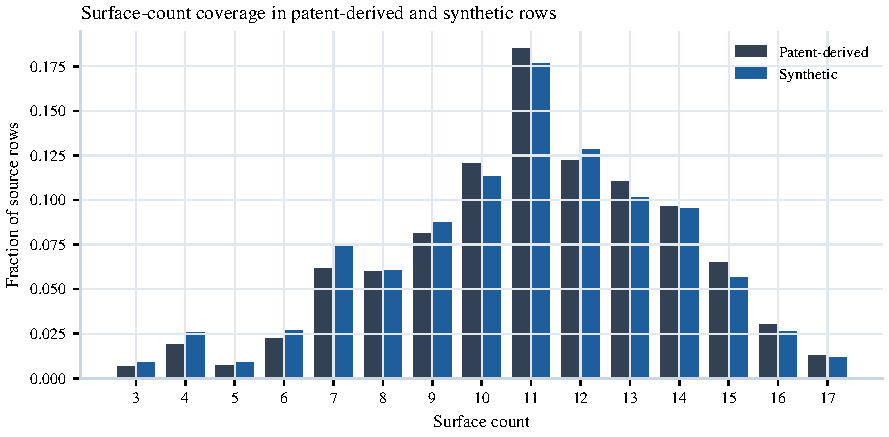
\includegraphics[width=0.88\linewidth]{figures/dataset_surface_count_distribution.pdf}
\caption{\textbf{Surface-count distribution.} Patent-derived and synthetic designs both span 3--17 active surfaces, with a median of 11. Bars show the fraction within each source type rather than raw counts.}
\label{fig:appendix_surface_count_distribution}
\end{figure}

\begin{figure}[htbp]
\centering
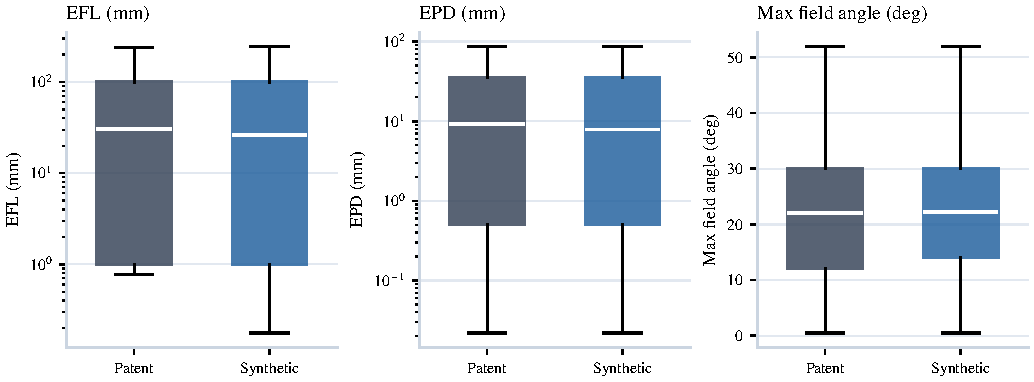
\includegraphics[width=0.9\linewidth]{figures/dataset_design_condition_distributions.pdf}
\caption{\textbf{Design-condition distributions.} Effective focal length, entrance-pupil diameter, and maximum field angle are compared between patent-derived and synthetic designs. The EFL and EPD axes are logarithmic.}
\label{fig:appendix_condition_distributions}
\end{figure}

\begin{figure}[htbp]
\centering
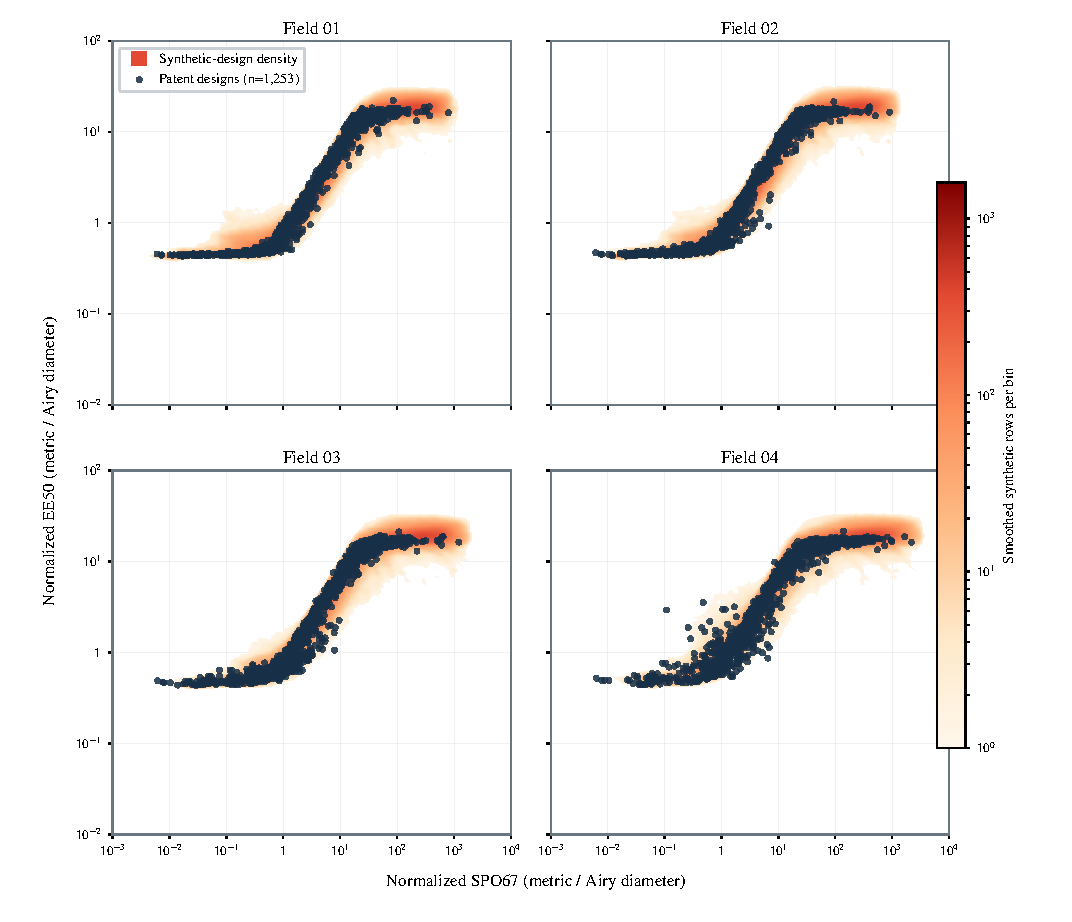
\includegraphics[width=0.95\linewidth]{figures/normalized_ee50_vs_spo67_remaining_fields_appendix.pdf}
\caption{\textbf{Off-axis optical-performance distributions.} Airy-normalized EE50 and SPO67 are shown at the four non-axial field positions. Patent designs are overlaid on the smoothed synthetic-design density, and both axes use logarithmic scaling.}
\label{fig:appendix_remaining_field_performance}
\end{figure}

\section{Model-Facing Dataset Details}

\subsection{Untuned and Tuned Representations}

Table~\ref{tab:tuned_untuned_representation} expands the distinction between the two model-facing representations summarized in Section~\ref{sec:canonical_model_representations}.

\begin{table}[htbp]
\centering
\small
\caption{Untuned and tuned model-facing representations. Both are derived from the same canonical rows and preserve row order and split labels.}
\label{tab:tuned_untuned_representation}
\begin{tabular}{@{}p{0.19\linewidth}p{0.35\linewidth}p{0.38\linewidth}@{}}
\toprule
\textbf{Quantity} & \textbf{Untuned representation} & \textbf{Tuned representation} \\
\midrule
Material & Catalog labels mapped to continuous $N_d$ and $V_d$ coordinates with air indicated explicitly. & The same continuous $N_d$ and $V_d$ coordinates and explicit air indicator. \\
Surface shape & Signed radius of curvature in physical units. & Signed curvature scaled by total system length. \\
Axial spacing & Inter-surface thickness in millimeters. & Valid inter-surface distances as axial fractions, with explicit system-length and image-gap terms. \\
Semi-diameter & Physical semi-diameter in millimeters. & Semi-diameter normalized by entrance-pupil diameter. \\
Aperture stop & Raw stop-surface index treated as categorical topology. & Stop position normalized by surface count and treated as a numerical topology variable. \\
Inactive surfaces & Structural missing values outside the active surface count. & The same structural missingness mask. \\
Inverse processing & Restores export defaults and the structural mask. & Inverts material, curvature, thickness, semi-diameter, and stop transforms before export and restores the structural mask. \\
\bottomrule
\end{tabular}
\end{table}

\subsection{Benchmark Split Source Counts}

Patent families are assigned to partitions before dataset-size variants are formed, keeping each patent and its synthetic descendants in one partition. The benchmark artifacts used for the reported models combine the canonical training and validation partitions into the model-training table; the test partition remains held out. Table~\ref{tab:canonical_split_source_breakdown} gives the resulting source counts. Synthetic validation and test rows are fixed across the 250k, 500k, and full variants; the size label counts sampled synthetic training rows only.

\begin{table}[htbp]
\centering
\footnotesize
\setlength{\tabcolsep}{4pt}
\caption{Patent-derived and synthetic rows in the benchmark training and held-out test tables.}
\label{tab:canonical_split_source_breakdown}
\begin{tabular}{lrrrrrr}
\toprule
\textbf{Variant} & \multicolumn{3}{c}{\textbf{Training rows}} & \multicolumn{3}{c}{\textbf{Held-out test rows}} \\
\cmidrule(lr){2-4}\cmidrule(lr){5-7}
 & \textbf{Patent} & \textbf{Synthetic} & \textbf{Total} & \textbf{Patent} & \textbf{Synthetic} & \textbf{Total} \\
\midrule
Patent-only & 1,128 & 0 & 1,128 & 125 & 0 & 125 \\
Patent+Synth-250k & 1,128 & 360,986 & 362,114 & 125 & 112,517 & 112,642 \\
Patent+Synth-500k & 1,128 & 610,986 & 612,114 & 125 & 112,517 & 112,642 \\
Patent+Synth-full & 1,128 & 1,012,563 & 1,013,691 & 125 & 112,517 & 112,642 \\
\bottomrule
\end{tabular}
\end{table}

\section{Benchmark Result Details}
\label{app:benchmark_result_details}

\subsection{Synthetic-Expansion Outcome Breakdown}
\label{app:section_6_1_failure_breakdown}

The main Section~\ref{sec:results_synthetic_expansion} reports feasible sample fractions for Patent-only and Patent+Synth-full training under the tuned representation with physics-based post-processing. Table~\ref{tab:appendix_section_6_1_failure_breakdown} provides the corresponding preparation and CodeV outcome breakdown. The outcome categories are computed over the same 10{,}000 generated rows per model/dataset/seed run and then averaged across four sampling seeds. Pre-CodeV rejected rows fail before submission to CodeV/LLESP, CodeV error rows are submitted but return with an error, and feasible rows are submitted and return successfully.

\begin{table}[htbp]
\centering
\scriptsize
\setlength{\tabcolsep}{4pt}
\caption{\textbf{Outcome composition for Section~\ref{sec:results_synthetic_expansion}.} Values are mean percentages of generated rows across four sampling seeds and sum to approximately 100\% for each row.}
\label{tab:appendix_section_6_1_failure_breakdown}
\begin{tabular}{llrrr}
\toprule
\textbf{Model} & \textbf{Training data} & \shortstack{\textbf{Pre-CodeV}\\\textbf{rejected}} & \shortstack{\textbf{CodeV}\\\textbf{error}} & \shortstack{\textbf{Feasible}\\\textbf{rows}} \\
\midrule
CoDi & Patent-only & 10.82 & 82.09 & 7.09 \\
CoDi & Patent+Synth-full & 4.69 & 38.74 & 56.57 \\
SMOTE-style reference & Patent-only & 0.00 & 13.16 & 86.84 \\
SMOTE-style reference & Patent+Synth-full & 0.18 & 1.52 & 98.30 \\
STaSY & Patent-only & 31.27 & 68.20 & 0.54 \\
STaSY & Patent+Synth-full & 6.84 & 16.66 & 76.50 \\
TabSyn ($3\times10^{-4}$) & Patent-only & 7.07 & 74.31 & 18.62 \\
TabSyn ($3\times10^{-4}$) & Patent+Synth-full & 1.55 & 14.73 & 83.72 \\
\bottomrule
\end{tabular}
\end{table}

\subsection{Ray-Tracing Post-Processing Metric Details}
\label{app:raytrace_metric_delta_details}

Section~\ref{sec:results_raytrace_postproc} reports the controlled ablation with and without physics-based post-processing using the seed-averaged paired heatmap and aggregate summary table. All distributions use the Patent+Synth-full TabSyn tuned run with diffusion learning rate $3\times10^{-4}$. Across the four sampling seeds, the branch without post-processing has 6{,}730 \ensuremath{\pm} 47 feasible rows and the branch with post-processing has 8{,}372 \ensuremath{\pm} 28 feasible rows out of the same 10{,}000 generated-row denominator. SPO and encircled-energy metrics are normalized by Airy diameter; nominal performance is left in its returned units.
